
\documentclass{article} % For LaTeX2e
\usepackage{iclr2027_conference,times}

% Optional math commands from https://github.com/goodfeli/dlbook_notation.
\input{math_commands.tex}

\usepackage{hyperref}
\usepackage{url}
\usepackage{xcolor}
\usepackage{xspace}
\usepackage{booktabs}
\usepackage{graphicx}
\usepackage{multirow}
\usepackage{makecell}


\title{\ourmethod{}: A Hierarchical Novelty-Aware Cascade for Multi-Cancer Liquid Biopsy Diagnosis}
% Global paper constants

\definecolor{Brown}{HTML}{6B3A32}
\definecolor{Red}{HTML}{A01822}

\newcommand{\ourmethod}{%
  % \textsc{
  \textcolor{Red}{Drop}\textsc{\textcolor{Brown}{Cascade}}\xspace%
}

\newcommand{\numsubtypes}{27}

% Authors must not appear in the submitted version. They should be hidden
% as long as the \iclrfinalcopy macro remains commented out below.
% Non-anonymous submissions will be rejected without review.

\author{Antiquus S.~Hippocampus, Natalia Cerebro \& Amelie P. Amygdale \thanks{ Use footnote for providing further information
about author (webpage, alternative address)---\emph{not} for acknowledging
funding agencies.  Funding acknowledgements go at the end of the paper.} \\
Department of Computer Science\\
Cranberry-Lemon University\\
Pittsburgh, PA 15213, USA \\
\texttt{\{hippo,brain,jen\}@cs.cranberry-lemon.edu} \\
\And
Ji Q. Ren \& Yevgeny LeNet \\
Department of Computational Neuroscience \\
University of the Witwatersrand \\
Joburg, South Africa \\
\texttt{\{robot,net\}@wits.ac.za} \\
\AND
Coauthor \\
Affiliation \\
Address \\
\texttt{email}
}

% The \author macro works with any number of authors. There are two commands
% used to separate the names and addresses of multiple authors: \And and \AND.
%
% Using \And between authors leaves it to \LaTeX{} to determine where to break
% the lines. Using \AND forces a linebreak at that point. So, if \LaTeX{}
% puts 3 of 4 authors names on the first line, and the last on the second
% line, try using \AND instead of \And before the third author name.

\newcommand{\todo}[1]{\textcolor{red}{TODO: #1}}


\begin{document}


\maketitle

\begin{abstract}
Multi-cancer early detection remains challenging because current diagnostic pathways often rely on invasive tissue biopsy, limiting repeated population-scale screening. Single-cell aptamer (APT) protein profiling offers a non-invasive liquid biopsy alternative, but clinically interpreting a single blood draw requires answering three nested questions: whether disease is present and which cancer type is involved (disease), how circulating immune cell lineages are distributed (lineage), and how fine-grained cell subtypes are composed (subtype). A reliable model should address these hierarchical predictions without becoming overconfident on cancer types or cellular states unseen during training. We introduce, to our knowledge, the first benchmark for hierarchical, novelty-aware classification on aptamer-based single-cell liquid biopsy data, together with \ourmethod{}, a hierarchical, novelty-aware cascade for multi-cancer characterization from a single blood draw, validated on this benchmark. Because disease-level prediction is near saturation under our protocol, a lightweight linear front end handles this level, while \ourmethod{} focuses on lineage and subtype prediction through differentiable soft routing over the lineage-subtype taxonomy with joint classification and novelty scores. This design identifies insufficient evidence for assigning cells to known categories rather than forcing closed-set predictions. We evaluate \ourmethod{} on a real-world multi-cancer APT dataset of 40 patients and more than 370,000 single cells using a strict patient-independent protocol with classical machine learning and neural baselines, patient-level bootstrap confidence intervals, and leave-one-disease-out (LODO) generalization tests. Under patient-level 5-fold cross-validation, \ourmethod{} matches or exceeds XGBoost in macro-F1 and improves coarse-fine prediction consistency to 82.8\%, compared with 73.6\% for XGBoost. Under a nested LODO training scheme, the novelty detection head achieves a mean AUROC of 0.81 and mean AUPR of 0.86 across six held-out disease groups for detecting cells from unseen diseases, outperforming a training-free confidence-based baseline with a mean AUROC of 0.63. These results demonstrate a unified approach to hierarchical prediction, patient-independent evaluation, and explicit novelty detection for small-sample, long-tailed classification in liquid biopsy and related clinical machine learning settings.
\end{abstract}


\section{Introduction}

Beyond transcriptomic profiling, single-cell technologies increasingly aim
to capture complementary molecular layers from the same cell, including
cell-surface protein states that RNA alone does not resolve. Aptamers offer
one route to this: short, selected oligonucleotide probes that bind surface
targets and, because their identity is itself a nucleic-acid sequence, can
be read out and paired with transcriptome sequencing on the same cell.
Apt-seq first demonstrated that jointly measured aptamer-binding and RNA
profiles resolve cell composition in defined cell-line mixtures
\citep{delley2018combined}. Subsequent work extended this along two
directions: Aptomics scaled aptamer-based profiling to proteins, glycans,
and RNA in clinical specimens, capturing tumor heterogeneity and T-cell
differentiation states \citep{wu2025aptomics}, while SPARK-seq combined
CRISPR perturbation with aptamer and RNA sequencing to identify and
kinetically characterize surface-binding targets \citep{luo2026spark}.
Together, these studies establish that APT measurements are feasible at
single-cell resolution, discriminate defined cell populations, and support
downstream biological characterization. What remains less established is
whether APT features on their own support reliable identification of a
cell's annotated identity -- an evaluation that determines what downstream
model development and clinical application this modality can support. As
single-cell APT data accumulates across patient cohorts, this capability
needs to be evaluated directly: which annotated cell identities can APT
features support in a patient who contributed no data to model
development, and does paired APT improve on a specified RNA-only
reference?

Two comparisons are needed to answer this question. First, low fine-subtype
performance does not establish a lack of APT information: parent-lineage
errors, candidate-set size, annotation ambiguity and the fitted model all
affect reconstruction. True-lineage decoding must therefore be compared
with a training-only prior given the same privileged lineage. Second, an
RNA+APT gain can reflect patient structure or coarse-lineage correspondence
rather than finer cell pairing. Shuffling APT within patient and then within
patient and lineage provides progressively more specific controls.

APT-Bench brings these comparisons into one clinical PBMC evaluation
setting: 361{,}792 paired cells from 40 participants, 293 APT measurements,
and a fixed five-lineage/27-subtype ontology. Five patient-disjoint folds
and subject-balanced pooled Macro-F1 define a common new-patient target.
Classical and neural APT-only models establish reference performance;
Soft-cascade is one hierarchy-aware reference rather than a separate
algorithmic contribution. Our contributions are:
\begin{itemize}
    \item \textbf{An APT cell-typing evaluation resource.}
    A fixed input panel, operational hierarchy, patient folds, explicit scoring
    units and reference predictions support comparisons on the same target.
    Complete data access and portable reproduction remain release requirements.
    \item \textbf{Within-lineage discrimination beyond a candidate-set prior.}
    The full-budget MLP reaches oracle fine F1 of 0.385 versus 0.180 for a
    conditional-proportion baseline. Matched-budget APT/RNA results reveal
    heterogeneous recoverability across lineages, rather than a uniform
    assay-resolution deficit inferred from coarse/fine scores.
    \item \textbf{An RNA-reference increment with a bounded interpretation.}
    Paired APT improves MLP fine F1 by \pairedMLPGainTwoK{} and
    \pairedMLPGainFiveK{} at two RNA widths.
    Its overall patient-by-lineage-shuffle contrast remains unresolved:
    improvement over these RNA references does not yet establish finer-grained
    pairing specificity.
\end{itemize}

The resulting findings concern recoverability under a specified cohort,
taxonomy and training recipe. RNA-derived annotations are not independent
biological truth, and an increment over a restricted RNA representation is
not evidence that RNA intrinsically lacks that information. Patient-disjoint
testing supplies the evaluation foundation, not evidence of blood-based
diagnostic validity.


\section{Related Work}

\paragraph{Single-cell aptamer profiling.} Existing single-cell aptamer studies address complementary goals in cell discrimination, biological characterization, and probe discovery \citep{xu2024aptamer, wu2024efficient}. Apt-seq jointly measured aptamer binding and transcriptomes in individual cells, demonstrating discrimination between human Ramos and mouse 3T3 cells from their binding profiles \citep{delley2018combined}. \citep{wu2025high} developed an integrative strategy termed Aptomics to profile cell-surface proteins, glycans, and mRNA, characterizing tumor heterogeneity in clinical samples and glycosylation changes associated with T-cell differentiation. Along a complementary direction, SPARK-seq integrates CRISPR-based surface-protein perturbations with single-cell mRNA and aptamer sequencing to identify aptamer–target relationships and characterize binding kinetics \citep{luo2026spark}. Building on these profiling capabilities and biological applications, APTBench focuses on the predictive use of a fixed APT panel: evaluating cell-identity prediction under a specified RNA-derived reference taxonomy in patients excluded from model development.

\paragraph{Cell annotation and hierarchical prediction.} Cell-type annotation methods assign molecular profiles to reference identities through supervised classification or reference-based matching, as exemplified by CellTypist \citep{dominguez2022cross} and SingleR \citep{aran2019reference}. At larger scales, scTab \citep{fischer2024sctab} studied cross-tissue annotation using donor-wise data splits, providing a precedent for evaluating predictions on unseen donors. In parallel, foundation models such as scGPT \citep{cui2024scgpt} and Geneformer \citep{theodoris2023transfer} learn representations from large collections of single-cell transcriptomes and adapt them to downstream tasks through fine-tuning. To accommodate related cell populations and differing annotation resolutions, CHETAH \citep{de2019chetah} and scHPL \citep{michielsen2021hierarchical} organize reference populations into classification hierarchies. Hierarchical cross-entropy (HCE) further incorporates ancestor--descendant relationships between cell labels into the training objective \citep{cultrera2026improving}. Drawing on these methodological foundations, APTBench evaluates classical classifiers and hierarchy-aware reference models with APT inputs and analyzes prediction errors across and within lineages. Separately, its true-lineage oracle supplies the reference lineage at test time to diagnose remaining subtype discrimination, with training-derived conditional priors receiving the same lineage information as controls. 

\section{Benchmark Setting}
\label{sec:data}

\begin{figure}[H]
\centering
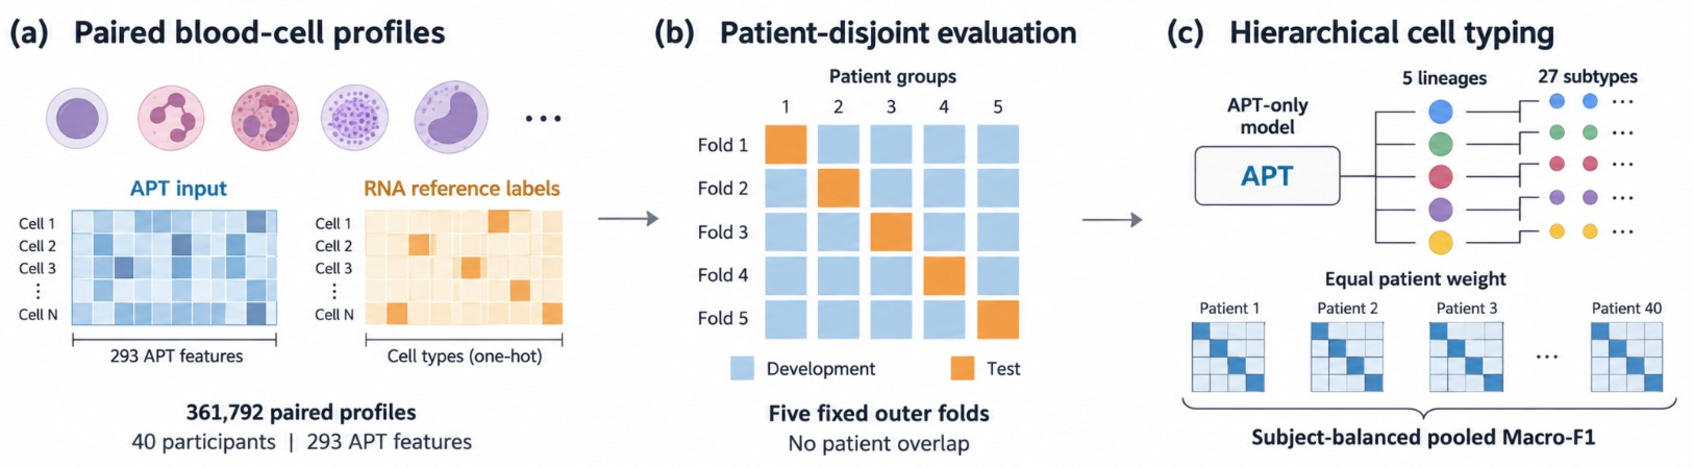
\includegraphics[width=\linewidth]{figures/cell_patient_overview.pdf}
\caption{The primary \ourbench{} contract. Patient-disjoint outer folds evaluate
cell typing in new individuals; subject-normalized confusion pooling assigns
equal total scoring weight to each patient.}
\label{fig:cell_patient_overview}
\end{figure}

\subsection{Blood Profiles and Reference Labels}
\label{sec:data:description}

\ourbench{} is derived from peripheral-blood specimens from \numparticipants{} participants in
five cancer groups (CRC, GC, HCC, PC, and BTC) and healthy controls, with 6--8
participants per group. The paired assay measures transcriptomic state and \numaptfeatures{}
aptamer features on the same cells. Transcriptomic counts
were processed with Seurat \citep{hao2021integrated}; predicted doublets and
low-quality cells were removed, and clusters were manually annotated using
canonical markers from prior PBMC and pan-cancer studies
\citep{mcginnis2019doubletfinder,zhang2024pan,yang2024pan}. These annotations
define \numlineages{} lineages and \numsubtypes{} subtypes. They are operational reference
labels, not independently measured biological truth.

The linked post-QC cohort contains 374{,}854 cells. Excluding the uncertain
\emph{Unknown} subtype leaves \numcells{} benchmark cells. Each subtype has one
fixed parent lineage. Disease is a six-class patient attribute, not the root of
the cell hierarchy: any given lineage can occur in multiple disease groups.
We evaluate the lineage-to-subtype hierarchy without imposing a
disease-to-lineage-to-subtype label tree. The construction checklist and
unresolved acquisition and annotation fields are recorded in
Appendix~\ref{sec:appendix:dataset_documentation}.

\subsection{Patient-Disjoint Cell-Typing Contract}
\label{sec:data:contract}
\label{sec:data:protocols}

The primary task is cell typing in new patients.
\textbf{Cell identity} predicts lineage and subtype using APT alone at inference.
Training supervision is recipe-specific: only Soft-cascade additionally uses
development-patient disease labels for contrastive pairing.
Open-set subtype discovery is outside the contract; all primary cell tasks
use the fixed five-lineage/27-subtype ontology.

\numfolds{} frozen disease-stratified folds each hold out eight patients. All cells
from a patient remain together. Benchmark-fitted transforms, model selection,
and fitting use development patients; the upstream provenance of the supplied
APT expression remains incompletely recovered
(Appendix~\ref{sec:appendix:main_protocols}). We pool predictions across the five
out-of-fold (OOF) partitions. The release
interface records cell and patient IDs, ontology, folds, predictions, and
metrics (Appendix~\ref{sec:appendix:benchmark_release}). Full data access and a
portable end-to-end evaluator remain release requirements.

\subsection{Metrics and Statistical Units}
\label{sec:data:imbalance}

Coarse and fine subject-balanced pooled Macro-F1 (SB-Macro-F1) are the primary
cell metrics. For patient $p$, let $C^{(p)}$ be the confusion matrix over a fixed
$K$-class ontology and $n_p$ its number of evaluated cells. Define
\begin{equation}
\overline C=\frac{1}{P}\sum_{p=1}^{P}\frac{C^{(p)}}{n_p},\qquad
\mathrm{SB\text{-}MacroF1}=\frac{1}{K}\sum_{k=1}^{K}
\frac{2\overline C_{kk}}{\sum_j\overline C_{kj}+\sum_i\overline C_{ik}}.
\label{eq:primary_sb_f1}
\end{equation}
A zero denominator contributes zero. Each patient's entire matrix, not each
class row, is normalized to unit mass. This differs from cell-weighted pooled
Macro-F1 and from mean within-subject Macro-F1. We retrospectively re-score the
frozen OOF predictions under this primary reporting convention; checkpoints
are not reselected.

Main-table intervals use 2{,}000 resamples and explicitly label their target:
P denotes patient uncertainty conditional on frozen fits, and SP additionally
resamples the three MLP training seeds. Each SP replicate averages three
seed-specific scores, using the same patient draw across them. Both are
pointwise and conditional on the fixed fold design; neither repeats model
selection. The comparison is descriptive, and an individual-score interval
is not a pairwise superiority test. Full resampling order is given in
Appendix~\ref{sec:appendix:identity_questions}.

The paired-RNA probe also uses subject-balanced pooled Macro-F1, but has a
different training budget and preprocessing protocol; its scores must not be
interpreted as additional architecture rows in the main table.
The experimental protocol is in Appendix~\ref{sec:appendix:identity_questions};
scoring-unit comparisons are in Appendix~\ref{sec:appendix:protocol_sensitivity}.


\section{Method}
\label{sec:method}

APT-Bench is intentionally broader than any single model. We nevertheless need a hierarchy-aware and novelty-aware reference architecture that can operate directly on APT profiles under the benchmark protocols. \ourmethod{} plays this role. It focuses on the genuine cell-level hierarchy, lineage $\rightarrow$ subtype, and leaves disease recognition to a separate lightweight front end.

\subsection{Cell Encoder}
\label{sec:method:backbone}

Each cell is represented by a standardized APT vector $x \in \mathbb{R}^{293}$. We embed feature identity and feature value separately. For aptamer index $i$, we form a token
\begin{equation}
t_i = \mathrm{Emb}(i) + \mathrm{MLP}_{\mathrm{val}}(x_i), \qquad i=1,\dots,293.
\end{equation}
A learnable \texttt{[CLS]} token is prepended to the resulting sequence and processed by a pre-norm Transformer encoder with 4 layers, 8 attention heads, hidden dimension 256, feed-forward dimension 512, GELU activations, and dropout 0.1. The final \texttt{[CLS]} representation
\begin{equation}
z = \mathrm{Encode}(x) \in \mathbb{R}^{256}
\end{equation}
serves as the shared cell representation for downstream tasks.

\subsection{Soft-Routed Hierarchical Cascade}
\label{sec:method:cascade}

Let $M=5$ be the number of coarse lineages and $K=\numsubtypes$ the number of fine subtypes. Each subtype $k$ belongs to exactly one parent lineage $m(k)$. A coarse head produces lineage logits
\begin{equation}
c = W_c z \in \mathbb{R}^{M},
\end{equation}
with routing distribution
\begin{equation}
p(m \mid x) = \mathrm{softmax}(c/\tau)_m,
\end{equation}
where $\tau=1$.

Instead of a hard cascade, which would force subtype prediction to follow only the top predicted lineage, \ourmethod{} uses a soft mixture of a global subtype path and lineage-specific experts:
\begin{equation}
s_k(x) =
\underbrace{g_k(z)}_{\text{global path}}
+
\alpha \, p(m(k)\mid x) \, e_{m(k),k}(z)
+
\gamma \log\!\big(\epsilon + (1-\epsilon)p(m(k)\mid x)\big),
\label{eq:cascade}
\end{equation}
Here $g(z)$ is a global subtype head, $e_{m,k}(z)$ is the expert associated with lineage $m$, $\alpha=1.0$, $\epsilon=0.1$, and $\gamma$ is ramped from 0 to 0.5 during early training. The global path prevents the model from collapsing to a hard hierarchy and allows recovery from coarse routing errors. Final predictions are
\begin{equation}
\hat{k} = \arg\max_k s_k(x),
\qquad
\hat{m} = \arg\max_m c_m.
\end{equation}

For analysis, we also compare soft routing with hard routing and oracle routing to separate errors caused by lineage uncertainty from those caused by subtype discrimination itself.

\subsection{Cross-Disease Contrastive Regularization}
\label{sec:method:contrastive}

We encourage subtype representations to align across disease contexts. Let
\begin{equation}
u = \frac{\mathrm{Proj}(z)}{\lVert \mathrm{Proj}(z) \rVert_2}
\end{equation}
be a normalized projection of the encoder representation. For anchor cell $i$, positives are cells with the same subtype but a different disease label. Same-subtype cells from the same disease are excluded because they do not test cross-disease invariance. Cells from different subtypes are treated as negatives, with additional emphasis on negatives that share the same coarse lineage. The contrastive loss weight is ramped from 0 to 0.2 after the early warmup period.

\subsection{Novelty Detection}
\label{sec:method:novelty}

Closed-set hierarchy prediction is insufficient for deployment because a new patient's cells may belong to a disease category absent from training. We therefore evaluate two novelty mechanisms.

\paragraph{Training-free scores.}
We first consider two standard training-free baselines. Given fine-level logits $s(x)$, we compute the maximum softmax probability novelty score
\begin{equation}
\mathrm{MSP}(x)
=
1-\max_k \mathrm{softmax}(s(x))_k
\end{equation}
\citep{hendrycks2016baseline}
and the energy score
\begin{equation}
\mathrm{Energy}(x)
=
-\log \sum_k \exp(s_k(x))
\end{equation}
\citep{liu2020energy}.
The same scores are computed from the lineage logits $c(x)$ to obtain coarse-level baselines.

\paragraph{Trained novelty head.}
For each LODO fold, we first train the encoder and cascade on the known diseases. We then freeze the representation and train a lightweight MLP novelty head on a proxy-novel disease selected from the known set:
\begin{equation}
\mathrm{NoveltyHead}: \mathbb{R}^{256} \rightarrow \mathbb{R}
\end{equation}
Cells from this proxy disease receive novelty label 1; cells from the remaining known diseases receive label 0. The true held-out disease is never used during either cascade training or novelty-head training. This nested design asks whether novelty learned from one simulated unseen disease transfers to a different truly unseen disease.

\subsection{Optimization and Model Scope}
\label{sec:method:training}

The classification cascade is trained jointly using
\begin{equation}
\mathcal{L}
=
\lambda_{\text{fine}}\mathcal{L}_{\text{fine}}
+
\lambda_{\text{coarse}}\mathcal{L}_{\text{coarse}}
+
w_{\text{contrast}}(t)\mathcal{L}_{\text{contrast}},
\end{equation}
where $\mathcal{L}_{\text{fine}}$ and $\mathcal{L}_{\text{coarse}}$ are cross-entropy losses with $\lambda_{\text{fine}}=1.0$ and $\lambda_{\text{coarse}}=0.5$. The contrastive weight increases to 0.2 according to the schedule in \S\ref{sec:method:contrastive}.

We optimize the cascade using AdamW with learning rate $10^{-4}$ and weight decay $10^{-5}$, gradient clipping at norm 1.0, batch size 512, and mixed-precision training. Models are trained for at most 50 epochs with early stopping based on validation fine-level macro-F1 with patience 10. The final configuration does not use class-balanced sampling, as our experiments found that it did not improve performance after correcting an implementation issue; additional details are provided in Appendix~\ref{sec:appendix:sampler}.

The novelty head is trained after the corresponding cascade checkpoint is fixed. We use AdamW with learning rate $10^{-3}$ and weight decay $10^{-4}$ for at most 30 epochs, with early-stopping patience 5. Disease recognition is not handled by a dedicated head inside \ourmethod{}. This is a deliberate modeling decision rather than a claim that disease is solved in a strong external sense: within-cohort disease prediction is already nearly saturated by simple classical baselines, while the architectural challenge addressed by \ourmethod{} is the unresolved cell-level hierarchy and novelty problem.


\section{Results}
\label{sec:results}

\subsection{Reference Performance in New Patients}
\label{sec:results:subtype_audit}

Table~\ref{tab:main} reports APT-only typing on the same 40 held-out patients.
Under the unified v2 protocol, fine SB-Macro-F1 is 0.134 for LR and XGBoost,
0.137 for MLP, 0.147 for Flat, 0.146 for HCE and 0.148 for Cascade without
disease supervision. The prespecified descriptive Flat-minus-MLP difference
is $+0.0100$ (paired 95\% CI $[-0.0047,0.0234]$), and Cascade-minus-Flat is
$+0.0011$ ($[-0.0093,0.0093]$). These intervals do not establish superiority
or equivalence. Models share input transforms, inner partitions and fresh
outer refits, but retain model-specific objectives and optimization budgets
(Appendix~\ref{sec:appendix:unified_v2}).

\begin{table}[H]
\centering\small
\setlength{\tabcolsep}{4pt}
\begin{tabular}{llcc}
\toprule
Model & CI & Fine SB-F1 $\uparrow$ & Coarse SB-F1 $\uparrow$ \\
\midrule
Logistic Regression & P & 0.134 [0.114, 0.146] & 0.296 [0.276, 0.315] \\
XGBoost & SP & 0.134 [0.118, 0.148] & 0.326 [0.304, 0.348] \\
Plain MLP & SP & 0.137 [0.121, 0.152] & 0.333 [0.307, 0.356] \\
Flat Transformer & SP & 0.147 [0.127, 0.162] & 0.342 [0.317, 0.365] \\
HCE Transformer & SP & 0.146 [0.126, 0.160] & 0.339 [0.316, 0.362] \\
Soft-cascade (no disease) & SP & 0.148 [0.129, 0.161] & 0.336 [0.311, 0.359] \\
\bottomrule
\end{tabular}
\caption{Unified v2 APT-only reference comparison on the same 361{,}792 OOF cells and 40 patients. All models use raw-count log1p inputs, training-only standardization, the same inner-patient split, and fresh refits on all 32 development patients. No main-table model uses disease supervision. Values are means across three training seeds (LR: one deterministic fit) with 5{,}000-resample pointwise 95\% intervals: P resamples patients; SP jointly resamples patients and seeds. LR/XGBoost select the two tasks separately; neural coarse scores are auxiliary outputs of fine-selected fits. HCE coarse scores use subtree probability mass. Model-specific search spaces and the selection-conditioned uncertainty target are given in Appendix~\ref{sec:appendix:unified_v2}.}
\label{tab:main}
\end{table}


\paragraph{Structure and extra supervision.}
Table~\ref{tab:unified_ablation} separates the full cascade structure from
cross-disease contrastive supervision. Adding contrastive supervision changes
fine SB-F1 by $+0.0006$ for Flat and $+0.0017$ for Cascade; their paired
intervals and the interaction interval include zero. This does not establish
that these recipes are equivalent or that hierarchy is unhelpful. In
particular, Cascade-minus-Flat changes the global/expert/routing combination,
not soft routing alone.
\begin{table}[t]
\centering\small
\setlength{\tabcolsep}{4pt}
\begin{tabular}{llcc}
\toprule
Recipe & Disease & Fine SB-F1 & Paired difference [95\% CI] \\
\midrule
A: Flat & No & 0.147 [0.127, 0.162] & --- \\
B: Flat & Yes & 0.148 [0.126, 0.163] & B$-$A: 0.0006 [-0.0057, 0.0071] \\
C: Cascade & No & 0.148 [0.129, 0.161] & C$-$A: 0.0011 [-0.0093, 0.0093] \\
D: Cascade & Yes & 0.150 [0.128, 0.166] & D$-$C: 0.0017 [-0.0087, 0.0123] \\
\bottomrule
\end{tabular}
\caption{Unified v2 $2\times2$ comparison of the whole cascade structure and cross-disease contrastive supervision. A and C reuse the main-table fits; B and D add the same contrastive term. Shared encoder, inputs and search rules are held fixed, but each recipe selects its own validation optimum. C$-$A is not a routing-only effect. The interaction (D$-$C)$-$(B$-$A) is 0.0012 [-0.0087, 0.0110]. Intervals are paired, pointwise and exploratory, not multiplicity-adjusted tests.}
\label{tab:unified_ablation}
\end{table}


\paragraph{Can predicted parents realize the oracle gain?}
Frozen-score diagnostics in Table~\ref{tab:unified_decoding} compare ordinary
subtype prediction with predicted-parent masking (D1), probability-consistent
combination (D2), and true-parent masking (D4). For the v2 MLP, fine SB-F1 is
0.137, 0.131, 0.134 and 0.376 respectively. Thus these two deployable readout
rules do not realize the oracle gain for this recipe. This is not a test of
all possible trained hierarchical classifiers. The prior-controlled analyses
below use their original, separately identified fits.

Five-lineage and 27-subtype tasks differ in cardinality, prevalence and label
boundaries. Their raw F1 difference alone does not identify an APT resolution
limit. The following prior-controlled comparisons instead ask what remains
recoverable within a known lineage. Full subtype reporting and the supporting
split-protocol comparison are retained in
Appendices~\ref{sec:appendix:subtype_audit} and
\ref{sec:appendix:protocol_sensitivity}.

\subsection{Within-Lineage Identity Is Recoverable, but Heterogeneous}
\label{sec:results:within_lineage}

True-lineage decoding masks each frozen fine score vector to the correct
parent's children. This is a privileged diagnostic, not a deployable prediction:
it supplies the reference parent at test time and narrows the candidate set.
We therefore compare it with training-only conditional priors and with a
stronger APT-only control that retrains after shuffling whole APT vectors within
each patient and true lineage. The shuffle preserves patient- and lineage-level
APT distributions while breaking each cell's original APT--subtype pairing.

Under the unified raw-count protocol, the MLP rises from 0.137 ordinary fine
SB-Macro-F1 to 0.376 with true-lineage decoding (Table~\ref{tab:apt_shuffle_signal}).
The corresponding patient-by-lineage-shuffled oracle is 0.216, giving a
real-minus-shuffled difference of $+0.160$ (95\% CI $[0.132,0.172]$);
the training-only conditional-proportion prior is 0.180. The Flat Transformer
replication gives a similar overall contrast, $+0.156$ ($[0.125,0.175]$).
Thus the oracle gain is not explained by candidate-set restriction or by the
preserved patient-by-lineage APT distribution alone. It supports cell-level
APT correspondence in this diagnostic setting, without identifying a molecular
mechanism or an assay information ceiling.

\begin{table}[t]
\centering\small
\setlength{\tabcolsep}{3pt}
\begin{tabular}{llcccc}
\toprule
Model & Scope & Real oracle & Shuffled oracle & Prior & Real $-$ shuffled \\
\midrule
MLP & All & 0.376 & 0.216 & 0.180 & \makecell{$+0.160$\\$[0.132,0.172]$} \\
Flat & All & 0.371 & 0.216 & 0.180 & \makecell{$+0.156$\\$[0.125,0.175]$} \\
\midrule
MLP & B & 0.469 & 0.182 & 0.193 & \makecell{$+0.288$\\$[0.229,0.321]$} \\
MLP & Myeloid & 0.265 & 0.111 & 0.124 & \makecell{$+0.155$\\$[0.125,0.182]$} \\
MLP & NK & 0.869 & 0.872 & 0.478 & \makecell{$-0.003$\\$[-0.011,0.004]$} \\
MLP & Other & 0.844 & 0.496 & 0.490 & \makecell{$+0.349$\\$[0.051,0.422]$} \\
MLP & T & 0.225 & 0.136 & 0.096 & \makecell{$+0.089$\\$[0.072,0.101]$} \\
\bottomrule
\end{tabular}
\caption{APT-only conditional-pairing diagnostic under true-lineage decoding
(fine SB-Macro-F1). Real APT keeps each cell's original APT vector; shuffled
APT retrains after permuting whole vectors within patient and true lineage in
each partition. The prior is the training-only conditional-proportion
expected-confusion baseline. MLP lineages are exploratory; Flat is the
prespecified overall replication. Intervals jointly resample patients,
training seeds and shuffle realizations. These privileged-label diagnostics
are not deployable scores.}
\label{tab:apt_shuffle_signal}
\end{table}


The signal is not uniform. For the MLP, the real-minus-shuffled oracle contrast
is positive for B, Myeloid, Other and T scopes, but unresolved and slightly
negative for NK ($-0.003$, $[-0.011,0.004]$), where real and shuffled oracle
scores are both high. This prevents a simple statement that every lineage
contains recoverable subtype information under APT. It instead shows that the
useful diagnostic signal depends on the parent lineage and its child taxonomy.

Error diagnostics explain why ordinary prediction remains difficult. Across
the v2 MLP, Flat, HCE and no-disease Cascade, roughly 73--74\% of ordinary
subtype errors cross parent lineages, and true-lineage decoding repairs about
64\% of those cross-parent errors. Even when the auxiliary coarse head predicts
the correct parent, the fine head still assigns an out-of-parent subtype for
14--18\% of such cells, showing imperfect coordination between the heads.
These are patient-balanced error rates, not additive components of Macro-F1.
Complete cross-model summaries and 27-by-27 ordinary/oracle matrices appear in
Appendix~\ref{sec:appendix:v2_failure_structure}.

Finally, a trained conditional subtype MLP asks whether this diagnostic signal
can be converted into deployable performance. The model uses a shared MLP
encoder, a lineage head, and within-lineage subtype heads trained only against
the true parent during training; at test time it predicts by
$q_{g(k)}(x)r_{k\mid g(k)}(x)$ without access to the true parent. Its ordinary
fine score is 0.138, compared with 0.137 for the ordinary v2 MLP
($+0.0008$, $[-0.0057,0.0056]$). Its true-lineage oracle score is 0.389,
but the deployable gain remains unresolved. The current evidence therefore
separates two statements: APT contains cell-level within-lineage signal under
the oracle diagnostic, and the simple conditional training recipe tested here
does not yet make that signal useful for overall deployed subtype prediction.

\paragraph{Does directly targeting the bottleneck help?}
We next keep the same MLP capacity and test fine-head parent-mass supervision,
coarse--fine consistency, privileged within-lineage distillation, and their
combinations (Table~\ref{tab:hbm_ablation}). A fresh reproduction of the v2 MLP
scores 0.136, close to the committed 0.137 reference. Distillation alone has
the largest new point estimate, 0.140; its paired difference from the reproduced
MLP is $+0.0040$ (95\% CI $[-0.0018,0.0087]$). Its overall cross-lineage error
does not fall ($+0.0011$, $[-0.0054,0.0068]$), and its oracle score rises more
than its ordinary score, so the hierarchy gap does not close. The full objective
scores 0.138 (difference $+0.0015$, $[-0.0025,0.0060]$) and changes cross-lineage
error by $+0.0045$ ($[-0.0005,0.0097]$). Its smaller oracle gap is driven mainly
by lower oracle performance (0.372 versus 0.378), not by the student approaching
the original oracle. Thus none of these objectives establishes a deployable
gain or reduces cross-lineage routing errors under the tested protocol.
\begin{table}[t]
\centering\small
\setlength{\tabcolsep}{3.2pt}
\resizebox{\linewidth}{!}{%
\begin{tabular}{lrrrrrr}
\toprule
Training objective & Fine & Coarse & Cross error & Outside $\mid$ coarse correct & Oracle & Gap \\
\midrule
Plain MLP & 0.136 & 0.335 & 0.491 & 0.176 & 0.378 & 0.242 \\
$+$ parent mass & 0.136 & 0.334 & 0.496 & 0.179 & 0.378 & 0.242 \\
$+$ parent mass $+$ consistency & 0.139 & 0.337 & 0.495 & 0.178 & 0.380 & 0.241 \\
$+$ distillation & \textbf{0.140} & 0.335 & 0.492 & 0.172 & 0.384 & 0.244 \\
$+$ parent mass $+$ distillation & 0.139 & 0.332 & 0.492 & 0.178 & 0.375 & 0.236 \\
Full HBM & 0.138 & 0.336 & 0.495 & 0.180 & 0.372 & 0.235 \\
\bottomrule
\end{tabular}}
\caption{Hierarchy-bottleneck mitigation with the unified MLP backbone.
Fine, coarse and oracle columns are subject-balanced Macro-F1; cross error is
the patient-balanced fraction of all predictions that are both wrong and
cross-lineage. Outside $\mid$ coarse correct is the fraction of cells whose
fine prediction leaves the true lineage among cells with a correct auxiliary
coarse prediction. Gap is oracle minus ordinary fine F1. Entries average three
matched seed slots over the same five patient folds. Oracle decoding supplies
the true lineage and is diagnostic, not deployable. Bold identifies the highest
deployable fine point estimate, not statistical superiority.}
\label{tab:hbm_ablation}
\end{table}


\begin{figure}[t]
\centering
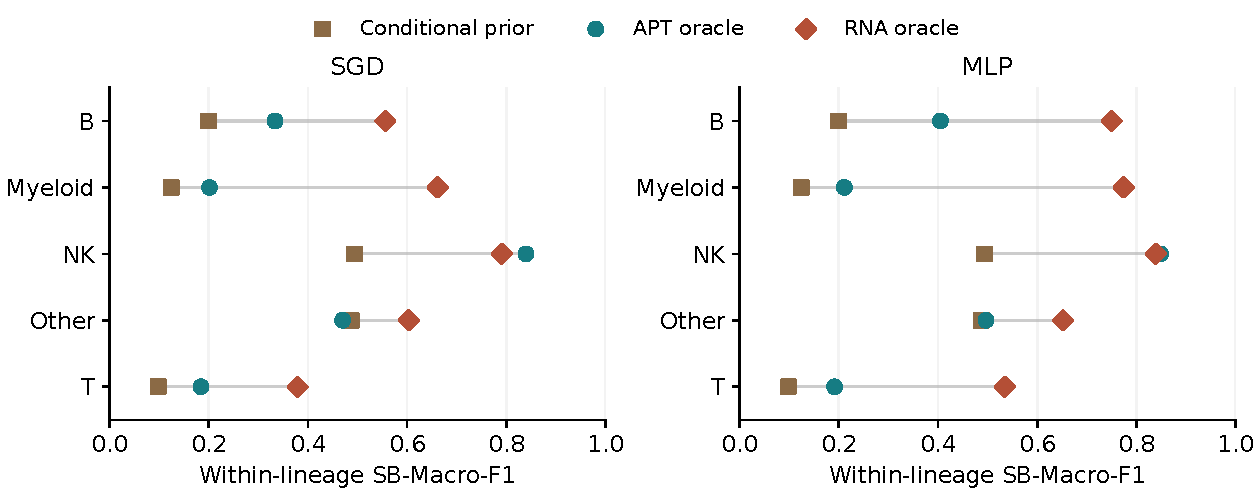
\includegraphics[width=\linewidth]{figures/matched_lineage_identity.pdf}
\caption{Matched-budget within-lineage reconstruction with 2,000
training-selected RNA HVGs. APT oracle, RNA oracle and conditional priors use
the same capped training subsets, patient folds and true-lineage information.
Points are means of three seed-specific scores, not F1 of seed-pooled
predictions; lines only connect methods within a lineage. Each patient's
matrix is normalized within the displayed lineage before pooling over
eligible patients and scoring its fixed children (38 patients for Other;
40 elsewhere). Consequently, these lineage scores cannot be averaged to
reconstruct the All row of Table~\ref{tab:matched_identity} from this same probe.
Row labels give the number of child subtypes.
These are descriptive point estimates, not superiority tests.
Expected-prior F1 is computed from an expected confusion matrix.}
\label{fig:matched_lineage_identity}
\end{figure}

The matched-input probe holds budget and recipe fixed across modalities
(Figure~\ref{fig:matched_lineage_identity}). MLP ordinary/oracle APT scores
are 0.093/0.309, RNA oracle is 0.672, and the expected prior is 0.182.
The APT oracle-minus-prior difference is $+0.127$ ($[0.101,0.139]$).
Relative to each lineage's own conditional prior and RNA reference,
APT reconstruction differs across lineages. Their absolute F1 values are
not a common biological-resolution scale: child-class counts and prevalence
also differ. For example, APT/RNA oracle scores are 0.849/0.839 for NK
but 0.191/0.535 for T cells. Knowledge of the parent therefore does not
uniformly resolve the RNA reconstruction gap. All lineages and both model
families are shown, without asserting an intrinsic modality ranking.

\paragraph{Budget and recipe matter.}
The full-budget MLP uses all development cells, a 256/128-unit network and
AdamW with selected stopping; the matched probe caps training at 1,000 cells
per patient and uses a 64-unit MLP for 40 epochs. Other has oracle F1 of
0.886 in the former but 0.497 in the latter (conditional expected priors
0.490/0.487). The recipes also differ in APT preprocessing
(Table~\ref{tab:identity_training_config}): log1p of raw counts in the matched
probe versus provided APT expression without an added log transform in the
full-budget MLP, each followed by training-set standardization.
Their score differences therefore cannot be attributed to training-cell budget alone.
Neither result justifies declaring Other universally identifiable or
unidentifiable. The full-budget lineage plot and neural-reference replays
are supporting evidence in Appendices~\ref{sec:appendix:full_budget_hierarchy}--\ref{sec:appendix:true_lineage_oracle}.

\subsection{Paired APT Improves on RNA, without Resolved Pairing Specificity}

Across three training seeds under the matched probe, MLP fine SB-Macro-F1 increases from 0.589 for RNA
to 0.607 for RNA+APT: $+\pairedMLPGainTwoK{}$ (joint 95\% CI $[0.009,0.030]$).
At 5,000 training-selected HVGs, it increases from 0.596 to 0.612:
$+\pairedMLPGainFiveK{}$ ($[0.009,0.029]$). SGD also improves at both widths
(Table~\ref{tab:paired_increment_main}). The increment is therefore not
specific to the 2,000-HVG setting, but remains relative to the tested RNA
representations and models.
Both widths use the capped-budget probe, not a full-cell-budget RNA model;
increasing HVGs does not control network capacity or training sufficiency.

\begin{table}[t]
\centering\small\setlength{\tabcolsep}{3pt}
\begin{tabular}{llcc}
\toprule
RNA HVGs & Comparator to paired RNA+APT & SGD $\Delta$ [95\% CI] & MLP $\Delta$ [95\% CI] \\
\midrule
2,000 & RNA & \makecell{$+0.0185$\\$[0.0034, 0.0332]$} & \makecell{$+0.0180$\\$[0.0092, 0.0297]$} \\
2,000 & RNA + noise & \makecell{$+0.0394$\\$[0.0240, 0.0537]$} & \makecell{$+0.0341$\\$[0.0208, 0.0448]$} \\
2,000 & Patient shuffle & \makecell{$+0.0059$\\$[-0.0049, 0.0165]$} & \makecell{$+0.0088$\\$[0.0014, 0.0145]$} \\
2,000 & Patient $\times$ lineage shuffle & \makecell{$+0.0064$\\$[-0.00437, 0.01657]$} & \makecell{$+0.0064$\\$[-0.00018, 0.01180]$} \\
\midrule
5,000 & RNA (width sensitivity) & \makecell{$+0.0217$\\$[0.0104, 0.0339]$} & \makecell{$+0.0165$\\$[0.0093, 0.0289]$} \\
\bottomrule
\end{tabular}
\caption{Overall fine SB-Macro-F1 differences, positive favoring paired
RNA+APT. Shuffle comparators append shuffled APT to RNA.
All 2,000-HVG contrasts use the same targeted experiment: three
training seeds and three realizations per seed for each shuffle type.
The 5,000-HVG row is the separate matched-width RNA comparison, not a
conditional-shuffle test. Scores are computed per fit before averaging;
2,000 paired seed/patient bootstrap replicates additionally resample shuffle
realizations where applicable. Intervals are pointwise and exploratory.
Both patient-by-lineage-shuffle intervals include zero.}
\label{tab:paired_increment_main}
\end{table}


\paragraph{What the controls establish.}
In the targeted 2,000-HVG experiment, MLP exceeds RNA+noise by 0.0341 and
patient-shuffled APT by 0.0088 (joint 95\% CI $[0.0014,0.0145]$).
This interval resamples patients, training seeds and shuffle realizations;
it is not a patient-only interval conditional on one fitted model.
The latter comparison uses three shuffle draws per
training seed, as does the more restrictive patient-by-lineage control.
Paired minus patient-by-lineage-shuffled APT is $+0.0064$
($[-0.00018,0.01180]$); SGD's corresponding interval also includes zero.
This is an unresolved overall contrast, not equivalence or evidence of no
pairing information. All control contrasts in the table come from the same
targeted experiment; the separate one-shuffle-per-seed width grid is labeled
as a sensitivity analysis in the appendix.
Lineage-specific contrasts remain exploratory supporting analyses
(Appendix~\ref{sec:appendix:identity_questions}).


\subsection*{AI use statement}

% (This section is \textbf{required} and does not count toward the page limit.)

% In this work, we used generative AI tools for [tasks with required disclosure].
% We have not used generative AI tools for [other tasks with required disclosure],
% and [the rest of the required disclosure tasks] are not applicable to this work.
% Additionally, we used generative AI tools for [tasks with recommended
% disclosure]. We have reviewed all AI-assisted work. [Elaborate. For example, “we
% checked LLM-generated research ideas for potential plagiarism through a manual
% literature survey”, “LLM-generated code was verified and tested for correctness
% by 2 authors”, etc.]. We take responsibility for the final content of this work,
% including text, claims or artifacts produced with the aid of generative AI.

% See the ICLR 2027 AI Policy for Authors for more details. This statement should
% not be more than 1 page.

\subsection*{Ethics statement}

% (This section is \textbf{recommended} and does not count toward the page limit.)

% If authors feel that their paper submission raises questions regarding the Code
% of Ethics, they are encouraged to include a paragraph of Ethics Statement (at
% the end of the main text before references) to address potential concerns where
% appropriate. Topics include, but are not limited to, studies that involve human
% subjects, practices to data set releases, potentially harmful insights,
% methodologies and applications, potential conflicts of interest and sponsorship,
% discrimination/bias/fairness concerns, privacy and security issues, legal
% compliance, and research integrity issues (e.g., IRB, documentation, research
% ethics). This statement should not be more than 1 page.

\subsection*{Reproducibility statement}


\subsubsection*{Author Contributions}

\subsubsection*{Acknowledgments}

\bibliography{iclr2027_conference}
\bibliographystyle{iclr2027_conference}

\appendix
\section{Appendix}

\subsection{Lineage-Resolved Disease-Specific Aptamer Signatures}
\label{sec:appendix:apt_markers}

To assess whether the APT panel captures molecular differences beyond cell-type composition, we examined, within each of the three major immune lineages (T/NK, B, and myeloid), the aptamer whose average expression was most enriched in a given disease relative to the other five groups (disease-specific aptamer, selected independently per lineage). Figure~\ref{fig:apt_markers} shows the resulting six disease-specific aptamers (one per disease category, including Normal) within each lineage. Several aptamers show a consistent, lineage-independent pattern: for example, the HCC-specific aptamer is elevated in HCC relative to all other categories in the T/NK, B, and myeloid compartments alike, suggesting a disease-associated signal that is not restricted to a single cell type. This lineage-resolved characterization is descriptive and based on the full panel prior to any train/test partitioning; it is intended to establish molecular plausibility for the APT modality rather than as a validated biomarker panel, and none of these aptamers are used as hand-selected features by \ourmethod{} or any baseline in \S\ref{sec:results}, which instead consume the full 293-dimensional panel.

\begin{figure}[h]
\centering
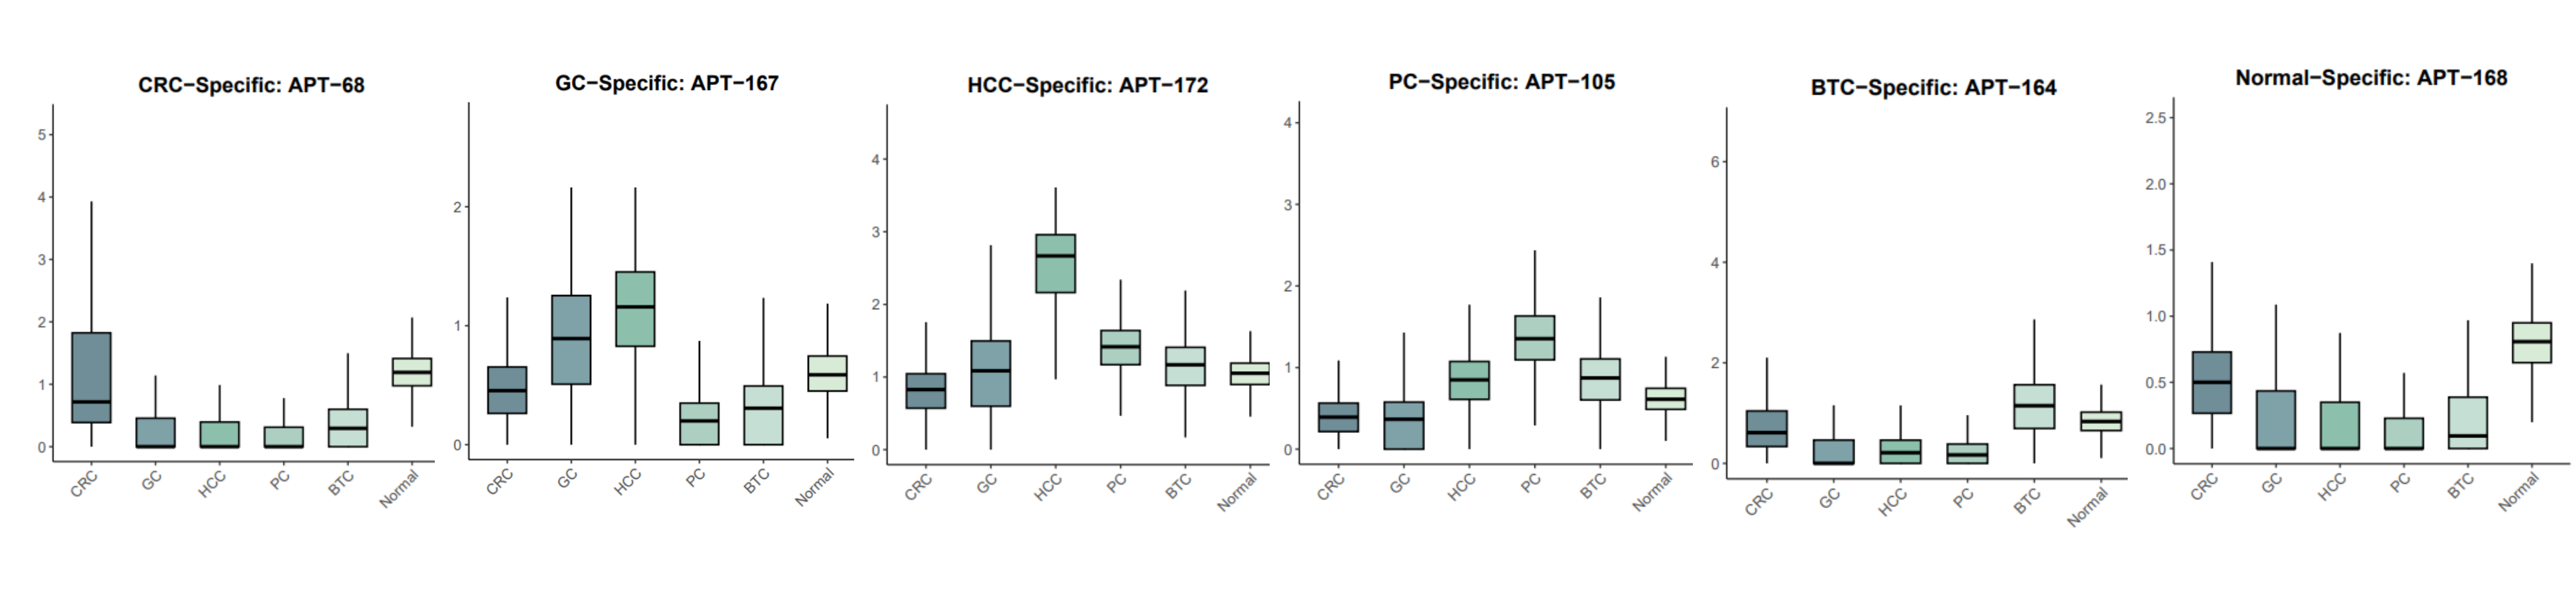
\includegraphics[width=\textwidth]{figures/apt_tnk_page-6_crop.png}
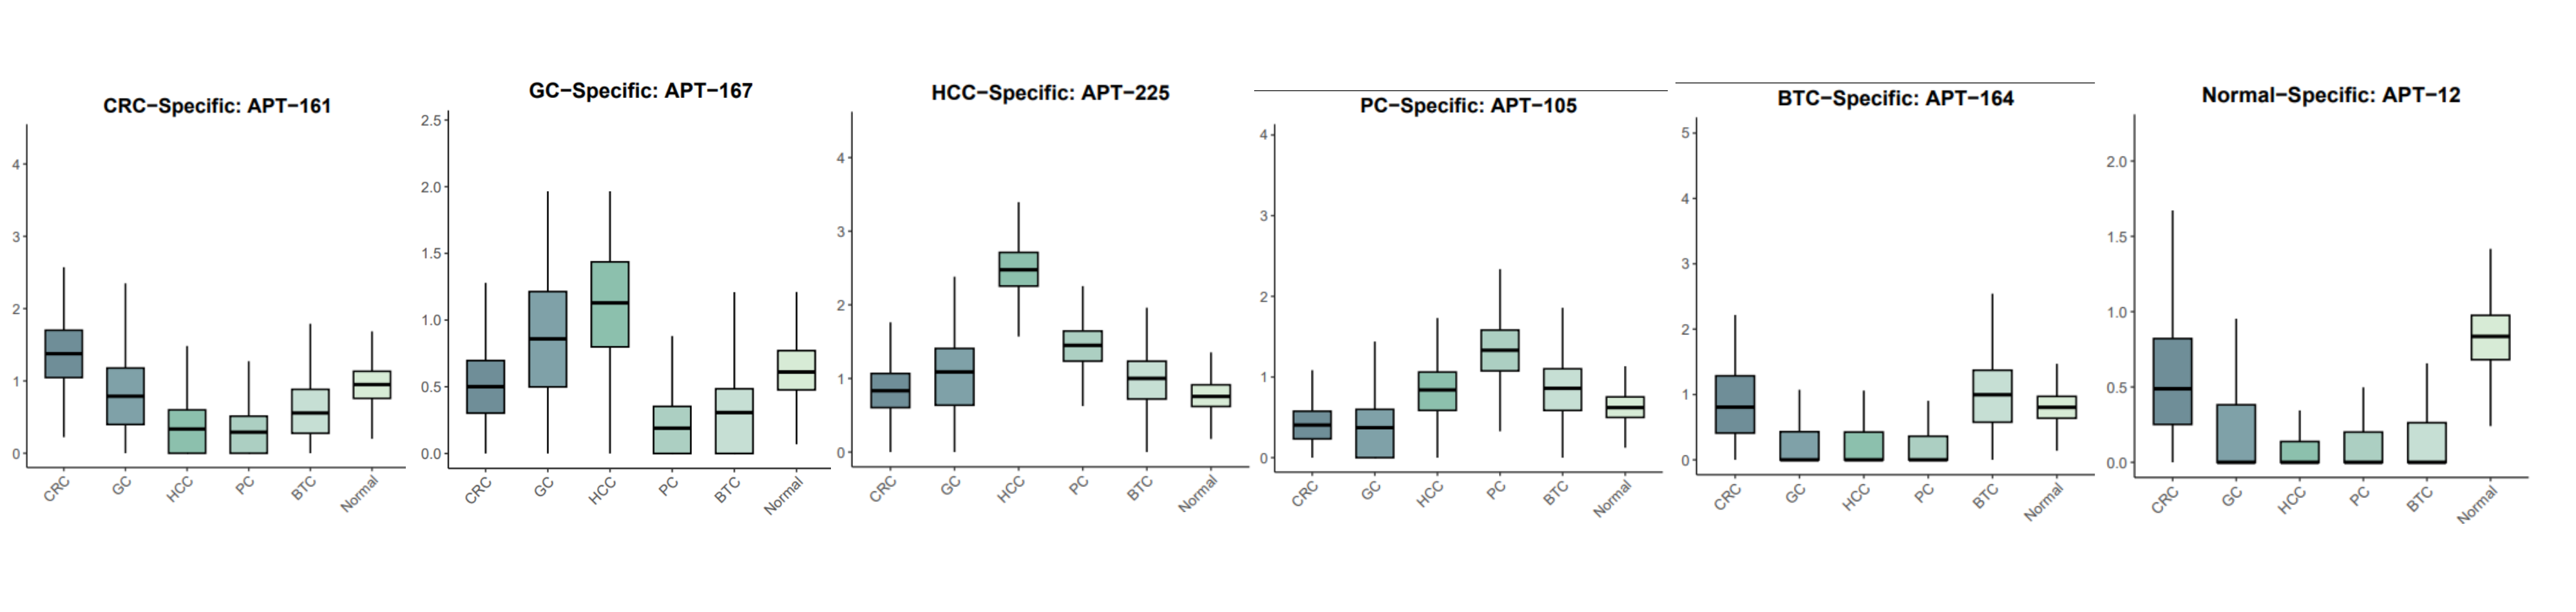
\includegraphics[width=\textwidth]{figures/apt_b_page-7_crop.png}
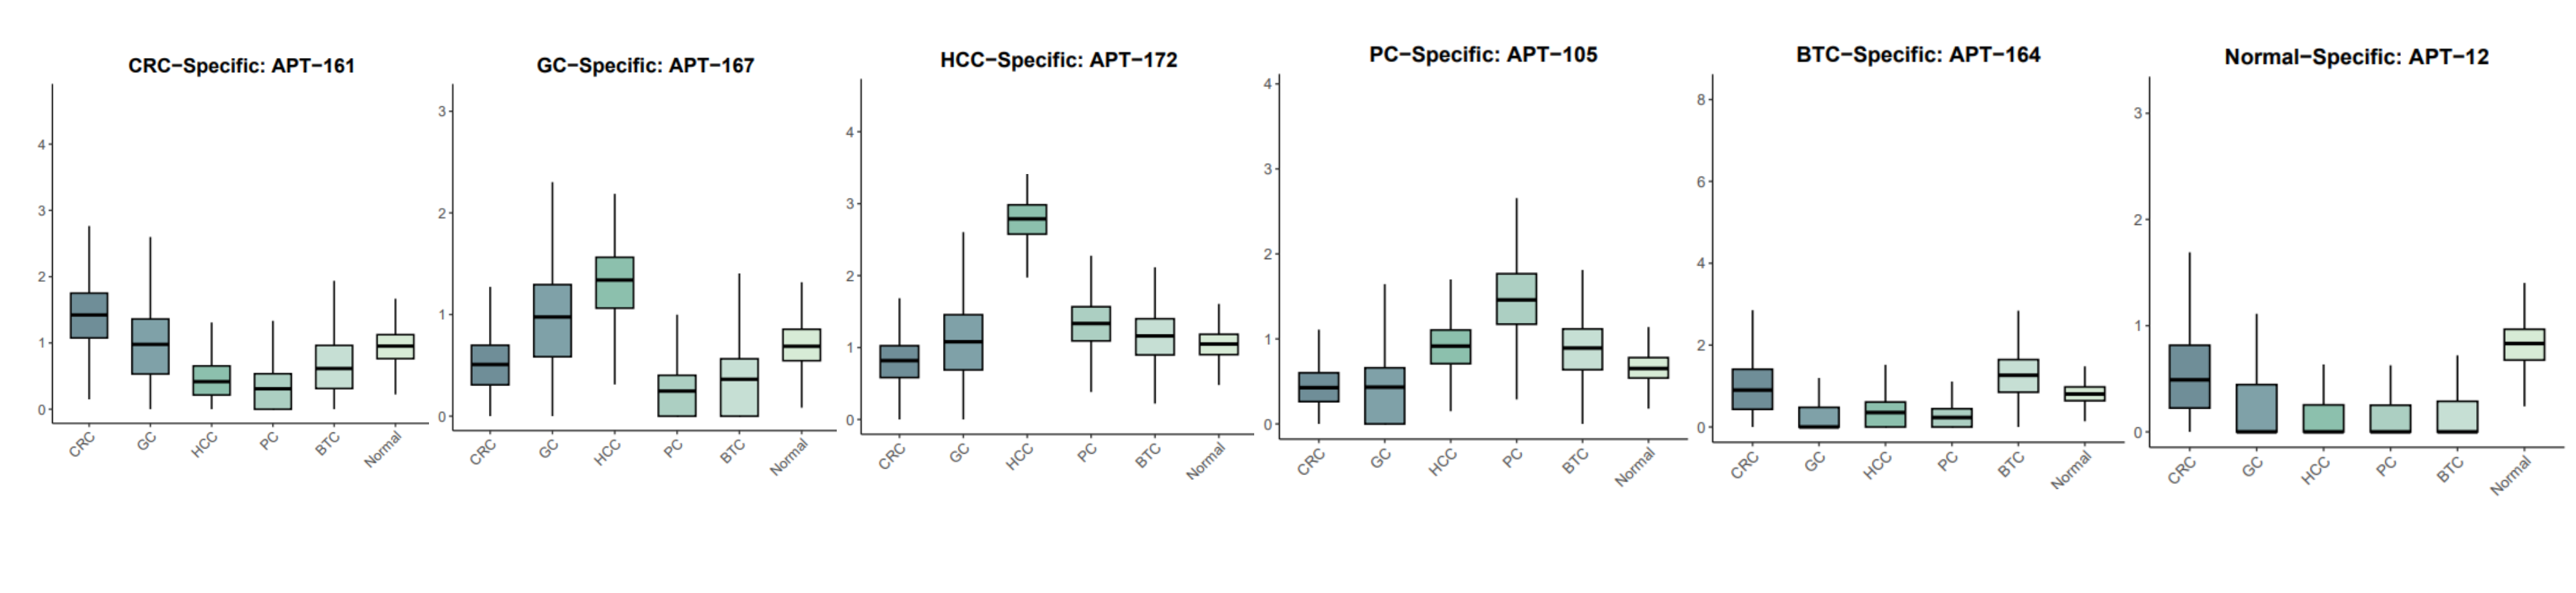
\includegraphics[width=\textwidth]{figures/apt_mono_page-8_crop.png}
\caption{Disease-specific aptamer expression (mean per-cell value, boxplots over cells) within the T/NK (top), B (middle), and myeloid (bottom) lineages. Each panel shows the aptamer most enriched in the named disease relative to the other five categories, computed independently within that lineage.}
\label{fig:apt_markers}
\end{figure}

\subsection{A Euclidean Heuristic Inspired by Hyperbolic Hierarchy Embedding}
\label{sec:appendix:hierarchy_margin}

Motivated by the observation that tree-structured label hierarchies can be embedded with lower distortion under hyperbolic geometry than Euclidean geometry \citep{nickel2017poincare}, we explored a lightweight Euclidean heuristic that directly enforces hierarchy-consistent distances between subtype representations, without the optimization overhead of a full hyperbolic parameterization (e.g., Riemannian optimization over a Poincar\'e ball). For each training batch we compute the mean encoder representation (\S\ref{sec:method:backbone}) of every subtype present in the batch as a prototype, and add a margin-based regularizer that penalizes same-lineage subtype prototypes farther apart than a margin $m_{\text{intra}}=1.0$ and different-lineage subtype prototypes closer together than a margin $m_{\text{inter}}=2.0$, added to the training objective (\S\ref{sec:method:training}) with weight $0.1$.

Under the single patient-independent split used for architecture development (\S\ref{sec:data:protocols}), this regularizer did not improve performance and in fact reduced it relative to the same configuration without the term: fine-subtype macro-F1 decreased from 0.171 to 0.136, and coarse-lineage macro-F1 decreased from 0.360 to 0.317. We did not conduct a hyperparameter sweep over the margin values or loss weight, so we cannot rule out that a different configuration would help; however, the result is consistent with the hierarchy-weighted term already present in the cross-disease contrastive loss (\S\ref{sec:method:contrastive}) capturing much of this signal, making an additional explicit hierarchy constraint redundant, or even conflicting, at this weight. We report this as a negative result rather than omitting it, and do not include this regularizer in the final \ourmethod{} configuration.

\subsection{Minimal Aptamer Panel for Disease Classification}
\label{sec:appendix:minimal_panel}

Because a smaller aptamer panel would be cheaper and simpler to deploy clinically, we ask how many of the 293 aptamers are actually needed for disease classification. We first rank all 293 aptamers by the absolute coefficient magnitude of an $\ell_1$-regularized multinomial logistic regression fit to the full cohort ($C=0.1$); this ranking step is used only to order features and is not used to report any performance number, so it does not leak into the evaluation below. For each candidate panel size $K \in \{5, 10, 15, 20, 30, 50, 75, 100, 150, 200, 293\}$, we restrict the APT input to the top-$K$ ranked aptamers and evaluate Logistic Regression and XGBoost under the same patient-level 5-fold protocol used throughout this work (\S\ref{sec:data:protocols}), reporting pooled out-of-fold disease macro-F1.

Figure~\ref{fig:panel_curve} shows the resulting panel-size--performance curve. Performance rises sharply with panel size and then plateaus: a panel of only 20 aptamers ($6.8\%$ of the full panel) already recovers $93\%$ of the full-panel macro-F1, and a panel of 50 aptamers ($17\%$) recovers $98\%$. Performance peaks around $K=150$--$200$ and does not further improve, and in fact is marginally lower at $K=293$ than at $K=200$ for both models, indicating that the full panel is not even performance-optimal for this task and that a substantially reduced panel is sufficient for disease classification. The top-20 ranked aptamers are APT-179, APT-225, APT-164, APT-166, APT-57, APT-125, APT-161, APT-69, APT-223, APT-172, APT-218, APT-167, APT-157, APT-54, APT-282, APT-47, APT-92, APT-196, APT-217, and APT-273.

This ranking, obtained purely from a discriminative model fit to predict disease labels, agrees closely with the descriptive lineage-resolved characterization in Appendix~\ref{sec:appendix:apt_markers}: 5 of the 6 disease-specific aptamers identified there independently (APT-172 for HCC, APT-225 for HCC, APT-164 for BTC, APT-167 for GC, and APT-161 for CRC) appear within this top-20 discriminative ranking, despite the two analyses using unrelated methodology (group-wise mean comparison versus $\ell_1$ coefficient ranking) and unrelated objectives (lineage-resolved marker discovery versus whole-panel disease classification). This convergence provides independent cross-validation that both analyses are identifying a shared, non-arbitrary subset of disease-informative aptamers rather than method-specific artifacts.

\begin{figure}[h]
\centering
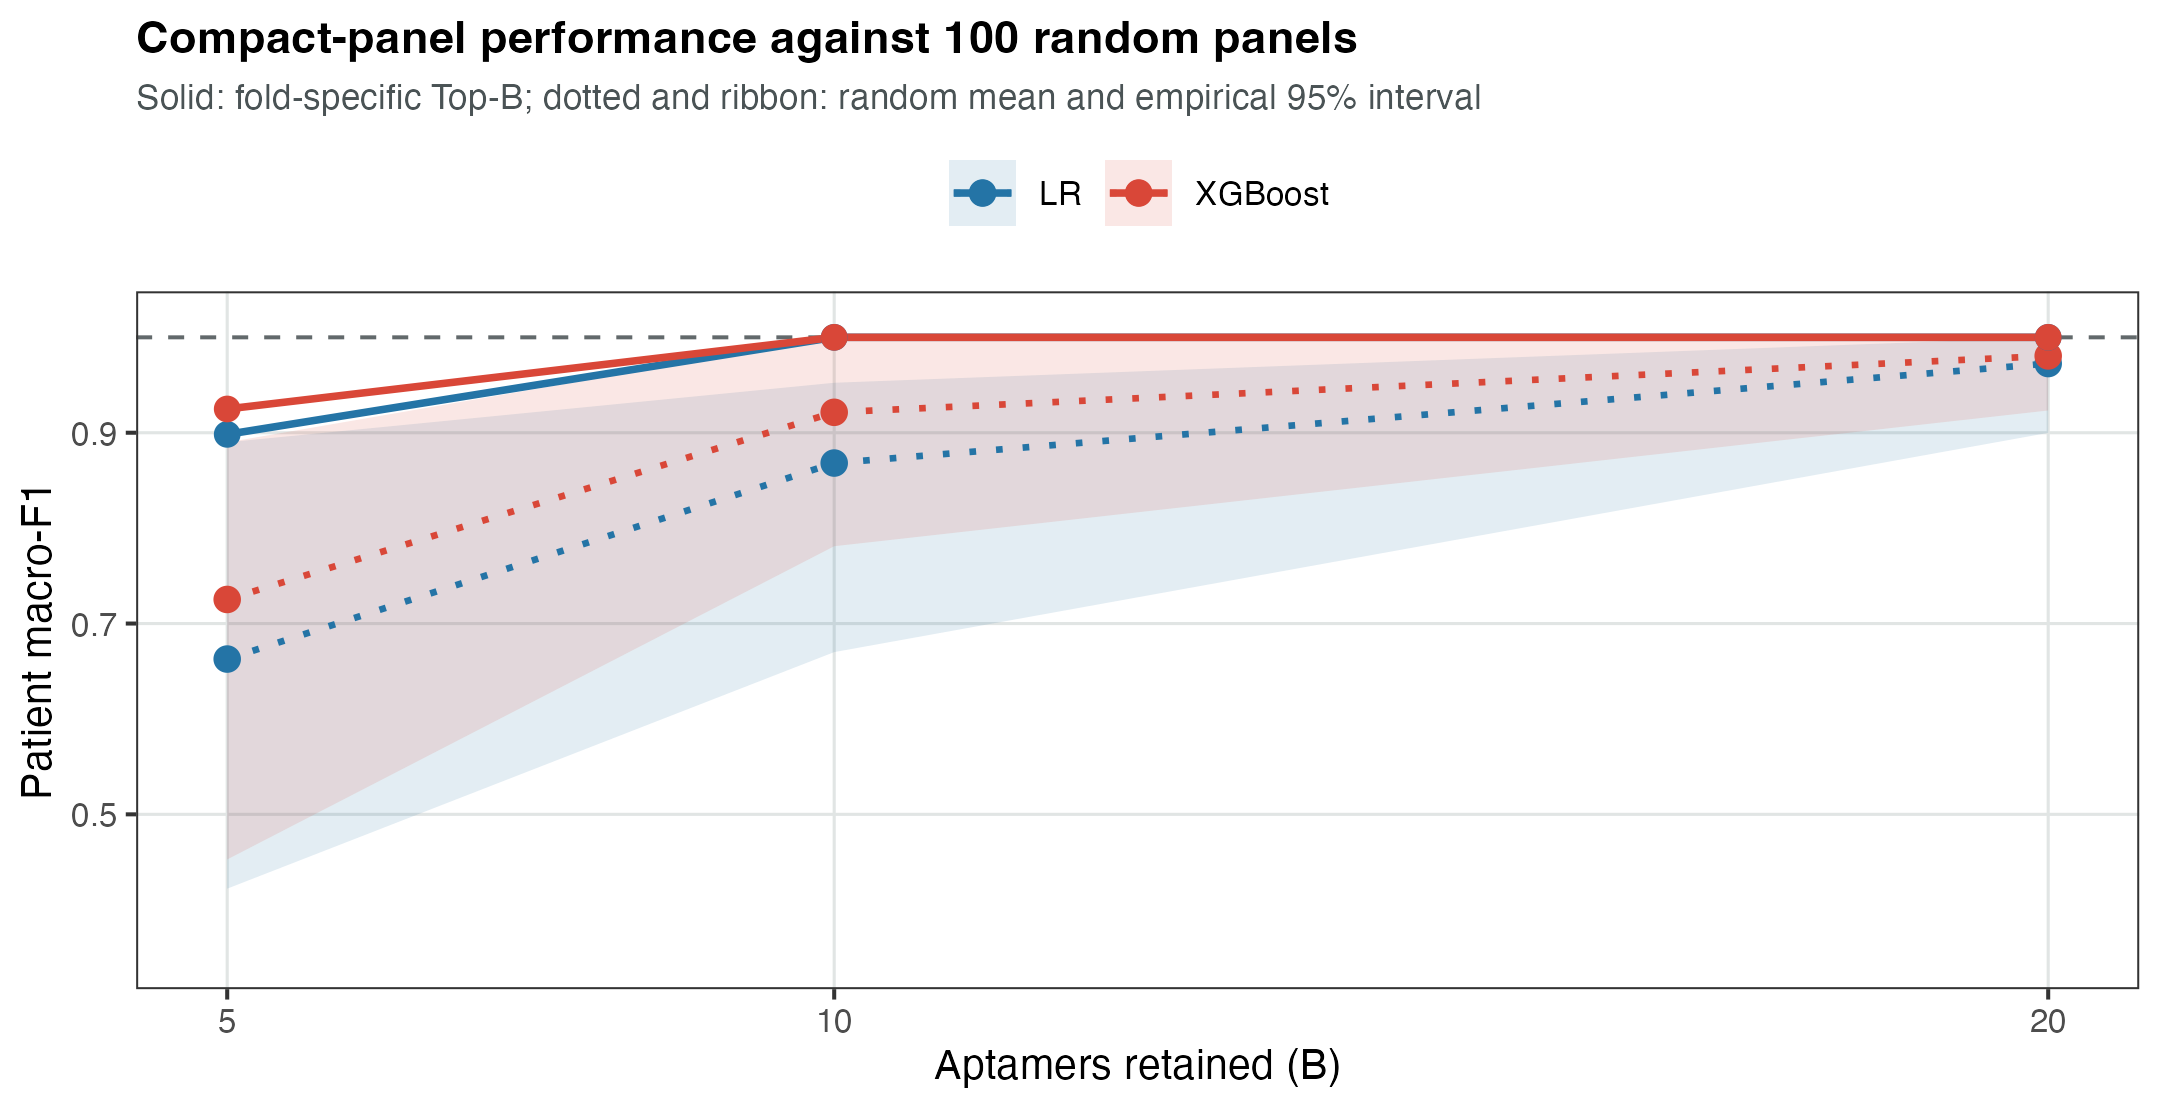
\includegraphics[width=0.7\textwidth]{figures/panel_size_curve.png}
\caption{Disease macro-F1 (pooled 5-fold, patient-independent) as a function of aptamer panel size, for panels restricted to the top-$K$ aptamers ranked by $\ell_1$-regularized logistic regression coefficient magnitude. The dashed line marks the full 293-aptamer panel's macro-F1.}
\label{fig:panel_curve}
\end{figure}

\subsection{Balanced Sampling Ablation}
\label{sec:appendix:sampler}

The final \ourmethod{} configuration (\S\ref{sec:method:training}) does not use class-balanced sampling. We initially implemented a balanced subtype-disease batch sampler to counteract the long-tailed subtype distribution (\S\ref{sec:data:imbalance}), but found and fixed an implementation issue in which \texttt{steps\_per\_epoch} was computed from the natural data loader's batch size (512) rather than the sampler's own, much smaller, per-batch cell count (e.g., $14$ subtypes $\times$ $2$ diseases $\times$ $4$ cells $= 112$); this mismatch caused each nominal epoch to cover only about $22\%$ of the training set when the sampler was enabled, silently under-training the model and desynchronizing every epoch-indexed schedule (warmup, contrastive ramp-up, routing ramp-up, early-stopping patience) relative to the sampler-disabled baseline.

After fixing this issue, the balanced sampler improved fine-subtype macro-F1 from $0.102$ to $0.119$ on the single patient-independent split used for architecture development, but both remain below the $0.171$ achieved without any balanced sampling at all. We report this ablation as a diagnostic finding about our specific sampler implementation, not as evidence against balanced sampling in general, and did not further redesign the sampler given this result; the final configuration therefore omits it.

\end{document}
